%!TEX encoding = UTF-8 Unicode
% ================================================================================
\documentclass[
    fontsize=12pt,
    headings=small,
    parskip=half,           % Ersetzt manuelles Setzen von parskip/parindent.
    bibliography=totoc,
    numbers=noenddot,       % Entfernt den letzten Punkt der Kapitelnummern.
    open=any,               % Kapitel kann auf jeder Seite beginnen.
%   final                   % Entfernt alle todonotes und den Entwurfstempel.
    ]{scrreprt}
% ===================================Praeambel==================================
% Kodierung, Sprache, Patches {{{
\usepackage[T1]{fontenc}    % Ausgabekodierung; ermöglicht Akzente und Umlaute
                            %  sowie korrekte Silbentrennung.
\usepackage[utf8]{inputenc} % Erlaubt die direkte Eingabe spezieller Zeichen;
                            %  utf8 muss die Eingabekodierung des Editors sein.
\usepackage[ngerman]{babel} % Deutsche Sprachanpassungen (z.B. Überschriften).
\usepackage{microtype}      % Optimale Randausrichtung und Skalierung.
\usepackage[
    autostyle,
    ]{csquotes}             % Korrekte Anführungszeichen in der Literaturliste.
%\usepackage{fixltx2e}      % Patches fuer LaTeX2e - seit 2015 nicht mehr nötig
\usepackage{scrhack}        % Verhindert Warnungen mit älteren Paketen.
\usepackage[
  newcommands
]{ragged2e}                 % Verbesserte \ragged...Befehle
\PassOptionsToPackage{
  hyphens
}{url}                      % Sorgt für URL-Umbrüche in Fußzeilen u. Literatur
% }}}

% Schriftarten {{{
\usepackage{mathptmx}       % Times; modifies the default serif and math fonts
\usepackage[scaled=.92]{helvet}% modifies the sans serif font
\usepackage{courier}        % modifies the monospace font
% }}}

% Biblatex {{{
\usepackage[
    style=alphabetic,
    backend=biber,
    %backref=true
    ]{biblatex}             % Biblatex mit alphabetischem Style und biber.
\bibliography{\jobname.bib} % Dateiname der bib-Datei.
\DeclareFieldFormat*{title}{
    \mkbibemph{#1}}         % Make titles italics
% }}}

% Dokument- und Texteinstellungen {{{
\usepackage[
    a4paper,
    margin=2.54cm,
    marginparwidth=2.0cm,
    footskip=1.0cm
    ]{geometry}             % Ersetzt 'a4wide'.
\clubpenalty=10000          % Keine Einzelzeile am Beginn eines Absatzes
                            %  (Schusterjungen).
\widowpenalty=10000         % Keine Einzelzeile am Ende eines Absatzes
\displaywidowpenalty=10000  %  (Hurenkinder).
\usepackage{floatrow}       % Zentriert alle Floats
\usepackage{ifdraft}        % Ermöglicht \ifoptionfinal{true}{false}
\pagestyle{plain}           % keine Kopfzeilen
% \sloppy                    % großzügige Formatierungsweise
\deffootnote{1em}{1em}{
  \thefootnotemark.\ }      % Verbessert Layout mehrzeiliger Fußnoten

\makeatletter
\AtBeginDocument{%
    \hypersetup{%
        pdftitle = {\@title},
        pdfauthor  = \@author,
    }
}
\makeatother
% }}}

% Weitere Pakete {{{
\usepackage{verbatim}
\usepackage{tikz}			% Für die Baumstruktur
\usetikzlibrary{positioning}
\usepackage[edges]{forest}
\usepackage{enumitem}        % style nextline für description
\usepackage{graphicx}       % Einfügen von Graphiken.
\usepackage{tabu}           % Einfügen von Tabellen.
\usepackage{multirow}       % Tabellenzeilen zusammenfassen.
\usepackage{multicol}       % Tabellenspalten zusammenfassen.
\usepackage{booktabs}       % Schönere Tabellen (\toprule\midrule\bottomrule).
\usepackage[nocut]{thmbox}  % Theorembox bspw. für Angreifermodell.
\usepackage{amsmath}        % Erweiterte Handhabung mathematischer Formeln.
\usepackage{amssymb}        % Erweiterte mathematische Symbole.
\usepackage{rotating}
\usepackage[
    printonlyused
    ]{acronym}              % Abkürzungsverzeichnis
\usepackage[
    colorinlistoftodos,
    textsize=tiny,          % Notizen und TODOs - mit der todonotes.sty von
    \ifoptionfinal{disable}{}%  Benjamin Kellermann ist das Package "changebar"
    ]{todonotes}            %  bereits integriert.
\usepackage[
    breaklinks,
    hidelinks,
    pdfdisplaydoctitle,
    pdfpagemode = {UseOutlines},
    pdfpagelabels,
    ]{hyperref}             % Sprungmarken im PDF. Lädt das URL-Paket.
    \urlstyle{rm}           % Entfernt die Formattierung von URLs.
%\usepackage{breakurl}
%\def\UrlBreaks{\do\/\do-}
\usepackage{listings}       % Spezielle Umgebung für Quelltextformatierung.
    \lstset{                
        language=csh,
        breaklines=true,
        breakatwhitespace=true,
        frame=l,            % Linie links: l, doppelt: L
		framerule=2.5pt,    % Dicke der Linie
		rulecolor=\color{gray},% Farbe der Linie
        captionpos=b,
        xleftmargin=6ex,
        tabsize=4,
        numbers=left,
        numberstyle=\ttfamily\footnotesize,
        basicstyle=\ttfamily\footnotesize,
        keywordstyle=\bfseries\color{green!50!black},
        commentstyle=\itshape\color{magenta!90!black},
        identifierstyle=\ttfamily,
        stringstyle=\color{orange!90!black},
        showstringspaces=false,
        morekeywords={  abstract, event, new, struct,
                as, explicit, null, switch,
                base, extern, object, this,
                bool, false, operator, throw,
                break, finally, out, true,
                byte, fixed, override, try,
                case, float, params, typeof,
                catch, for, private, uint,
                char, foreach, protected, ulong,
                checked, goto, public, unchecked,
                class, if, readonly, unsafe,
                const, implicit, ref, ushort,
                continue, in, return, using,
                decimal, int, sbyte, virtual,
                default, interface, sealed, volatile,
                delegate, internal, short, void,
                do, is, sizeof, while,
                double, lock, stackalloc,
                else, long, static,
                enum, namespace, string}
        }
%\usepackage{filecontents}  % Direktes Einfügen von Dateiinhalt. Wird hier für
                            %  die Verwendung einer .bib-Datei in dieser .tex-
                            %  Datei benötigt.
% }}}

% ===================================Dokument===================================

\title{Entwicklung eines Visualisierungswerkzeuges zur Demons-
tration datenschutzfreundlicher Dokumentspeicherdienste}
\author{David Kirchhausen Monteiro}

\begin{document}

\begin{titlepage}% {{{

\includegraphics[width=6.8cm]{../pic/up-uhh-logo-u-2010-u-farbe-u-rgb.pdf}
\begin{center}\Large
	% Universität Hamburg \par
	% Fachbereich Informatik
	\vfill
	Bachelorarbeit
	\vfill
	\makeatletter
	{\Large\textsf{\textbf{\@title}}\par}
	\makeatother
	\vfill
	vorgelegt von
	\par\bigskip
	\makeatletter
	{\@author} \par
	\makeatother
	geb. am 24. Januar 1994 in Hildesheim \par
	Matrikelnummer 6530927 \par
	Studiengang Software-System-Entwicklung
	\vfill
	\makeatletter
	eingereicht am {\@date}
	\makeatother
	\vfill
	Betreuer: Maximilian Blochberger, M. Sc. \par
	Erstgutachter: Prof. Dr.-Ing. Hannes Federrath \par
	Zweitgutachter: Tilmann Stehle, M. Sc.
\end{center}
\ifoptionfinal{}{}
\end{titlepage}% }}}
\chapter*{Aufgabenstellung}

Im  Zuge  dieser  Bachelorarbeit  soll  ein  einfacher  Dokumentenspeicher  entwickelt  werden,
welcher möglichst viele Nutzerdaten erfasst und speichert. Die erfassten Daten sollen anschaulich
grafisch dargestellt werden können. Weiter sollen verschiedene Szenarien entwickelt werden,
welche aufzeigen wie eine mögliche Benutzung des Services mit und ohne der Verwendung
von datenschutzfreundlichen Methoden zum Anonymisieren von Daten aussieht. Anhand der
Szenarien soll eine grafische Auswertung Unterschiede zwischen anonymisierten Daten und
nicht anonymisierten Daten visuell sichtbar machen und die Unterschiede somit leicht zugänglich
sein.

\chapter*{Zusammenfassung}
\begin{enumerate}
\item Dokumentenspeicherdienste Vorteile (Problemstellung erläutern)
\item Mögliche Datenschutz unfreundliche Aspekte von gängigen Anbietern (Problemstellung erläutern)
\item Entwicklung des Dokumentenspeichers und der Visualisierung zur deutlich Veranschaulichung von Potentiellen Unterschieden zwischen der Verwendung von Datenschutz freundlichen Methoden zum Anonymisieren oder nicht. (Bearbeitung der Problemstellung)
\begin{enumerate}
\item Implementation des Dokumentenspeichers
\item Implementation der API zur Datenübergabe 
\item Implementation des Visualisierungswerkzeug
\item Darstellung der Szenarien zur Benutzung des Visualisierungswerkzeug
\end{enumerate}
\end{enumerate}

\tableofcontents

\chapter{Einleitung}

Dokumentenspeicherdienste sind nützliche Alltagsgegenstände, welche für private sowie kommerzielle Nutzer meist unverzichtbar sind. 
Sie bieten nicht nur den Speicherplatz für wichtige Dateien der Nutzer sondern stellen auch die Sicherheit der Dateien sicher und machen sie global jederzeit verfügbar. 
Durch die große Datensammlung dieser Dienstleister machen sie sich nicht nur selbst zu lukrativen Zielen von gezielten Angriffen (Yahoo, UBER etc.), jedoch auch die Dienstleister selber können die Daten auswerten und weitere Metadaten wie z.B. die Dateigröße oder den Autor der Datei sowie Verkehrsdaten wie z.B. die IP-Adresse oder die HTTP Header Felder über die Nutzer sammeln und weiterverwenden. 
Vor allem private Nutzer sind meist gar nicht über die Risiken und das Missbrauchspotenzial aufgeklärt, welche die Verwendung solcher Dienstleistungen mit sich bringen. 
Methoden zur Verschlüsselung oder das anonymisieren von Daten sind Benutzern meist nicht bekannt, werden von den Dienstanbietern nicht angeboten oder sind schwer umzusetzen, da es einen meist erheblichen Aufwand für die Benutzer bedeutet und Kompetenzen erfordert welche diese Benutzer nicht besitzen. 
Um genau die Risiken und Missbrauchspotenziale aufzuzeigen wird im Zuge dieser Arbeit ein Dokumentenspeicherdienst entwickelt, welcher Meta- und Verkehrsdaten der Nutzer sammelt und diese in einer visuellen Darstellung zusammenfasst. 
Zur Implementation des Dokumentenspeichers wird dabei das Microsoft ASP.NET Core Framework verwendet. 
Das Framework wird benutzt um die Webbenutzeroberfläche sowie die Web API des Dokumentenspeichers zu realisieren. 
Dazu wird das Javascript Framework Data-Driven Documents, i.d.R. d3.js genannt, zur Visualisierung der Daten verwendet. 
Der Dokumentenspeicher soll vor allem den Unterschied zwischen der Verwendung von Methoden zur Verschlüsselung oder das anonymisieren von Daten visualisieren und verwaltet dazu zwei verschiedene Datensätze, wobei eine Datenmenge ohne, und eine Datenmenge mit der Verwendung von Methoden zur Verschlüsselung oder das anonymisieren von Daten erzeugt wird. Der entstehende Unterschied der gesammelten Metadaten durch die verschiedenen Methoden führt dann zu einer Veränderung in der Visualisierung, was dann den Effekt und Nutzen der Methoden deutlich sichtbar macht.  

\chapter{Grundlagen}

\section{Verwendungszweck des Dokumentenspeichers}
Der Dokumentenspeicher dient vor allem dazu den Vergleich zwischen den unterschiedlichen gesammelten Metadaten mit und ohne die Verwendung von datenschutzfreundlichen Methoden zum Anonymisieren von Daten. 
Diese entstehenden Unterschiede werden in der Visualisierung der Daten deutlich und veranschaulichen so den Effekt der Verwendung von datenschutzfreundlichen Methoden zum Anonymisieren von Daten.
Die durch datenschutzfreundlichen Methoden zum Anonymisieren von Daten erzeugte Datenmenge wird folgend als geschützte Datenmenge beschrieben und nimmt an, dass mindestens eine Methoden zum Anonymisieren von Daten benutzt wurde, um diese Datenmenge zu generieren. 
Die erzeugte Datenmenge ohne die Verwendung von datenschutzfreundlichen Methoden zum Anonymisieren wird folglich als ungeschützte Datenmenge beschreiben und nimmt an das keine Methoden zum Anonymisieren von Daten benutzt wurde oder der zumindest keine Methoden zum Anonymisieren von Daten verwendet wurde im Aspekt auf die Eigenschaften, die in einem gegebenen Szenario untersucht wurden.
Der Dokumentenspeicher ist somit so konzipiert, dass ein geschützter und ein ungeschützter Datensatz angelegt werden kann. 
Dafür wurden verschiedene API-Endpunkt implementiert, welche die Trennung der beiden Datensätze ermöglicht. 
Es können jedoch auch geschützte und ungeschützte Daten in die gleiche Datenmenge eingespeist werden, falls dies für das zu betrachtende Szenario sinnvoll ist. 
Die folgenden vorgestellten Szenarien trennen jedoch die geschützte Datenmenge und die ungeschützte Datenmenge und verwenden die dafür vorgesehenen API-Punkte.
Da die geschützte und ungeschützte Datenmenge verglichen werden soll, um den Effekt der zu untersuchenden Methode zum Anonymisieren von Daten sichtbar zu machen, ist es von Vorteil wenn die verwendeten Daten zum Erzeugen der geschützten und ungeschützten Datenmenge dieselben sind und sich lediglich durch die Anonymisierung der Daten und deren Effekt unterscheiden.
Dies stellt sicher, dass lediglich der Effekt der Methode zum Anonymisieren einen Unterschied in der Visualisierung erzeugt und keine anderen Faktoren die Visualisierung beeinflussen.
Im ideal Fall können so, durch die Betrachtung der Visualisierung der ungeschützten Datenmenge, Relationen zwischen Dateien deutlich werden, welche darauf schließen lassen, dass diese Dateien z.B. von dem gleichen Benutzer stammen.
Die Betrachtung der geschützten Datenmenge sollte dann im ideal Fall zeigen, dass durch die Verwendung von einer oder mehreren Methoden zum Anonymisieren von Daten diese Relation nicht mehr sichtbar ist und die Methode somit einen sichtbaren Effekt hat.

\newpage
\section{Terminologie}
\begin{enumerate}
\item HTTP-Header
\begin{enumerate}
\item Teil des Hypertext Transfer Protocol (HTTP)
\item Headerblock und Headerfeld nach RFC 2616(https://tools.ietf.org/html/rfc2616)
\end{enumerate}
\item Geo lookup
\begin{enumerate}
\item eine Methodik zur Bestimmung des geografischen Standort einer IP-Adresse
\item keine eigenen Implementation der Standortbestimmung, sondern Verwendung eines öffentlich zugänglichen Service, aus Zeit und komplexitätsgründen
\item Patent US7752210B2
\end{enumerate}
\item Header Fingerprint
\begin{enumerate}
\item eine Methodik zur Identifikation eines Benutzers anhand der von ihm Verwendeten HTTP Header
\item Aggregation über allen Http-Header oder einem ausgewählten Set an Headerfeldern 
\item erzeugt Fingerprint wird gehasht und gespeichert
\item bei übereinstimmenden Fingerprints wird angenommen das diese vom gleichen Benutzer erzeugt wurden 
\end{enumerate}
\end{enumerate}

%\newpage
%\section{Set A / Set B}
%
%Die angeführten DbSets FileEntryItemsA und FileEntryItemsB verfügen jeweils über Daten welche zu visualisieren sind. Dabei wird das DbSet FileEntryItemsA weiterhin als die ungeschützte Datenmenge beschrieben, da diese Datenbank nur mit Daten befüllt werden soll, bei welchen keine datenschutzfreundlichen Methoden zum anonymisieren verwendet wurden. Das DbSet FileEntryItemsB wird weiterhin als geschützte Datenmenge beschrieben, da ausschließlich Daten , welche mit Methoden zum anonymisieren hochgeladen wurden, verwendet werden sollen. Dabei sollte die geschützte und ungeschützte Datenmenge in den Zugrunde liegenden Datenmenge identisch sein und lediglich die Verwendung von Methoden zum anonymisieren die Datensätze unterscheiden, sodass die beiden Datenmenge miteinander in Hinblick auf den Effekt der Verwendung von Methoden zum anonymisieren untersucht werden können. 
%So wird im jedem beschriebenen Szenario zur Benutzung des Dokumentenspeichers angenommen das ein Benutzer eine Datei einmal ohne die Verwendung von Methoden zum anonymisieren in die ungeschützte Datenmenge via HTTP hochlädt und einmal mit der Verwendung von Methoden zum anonymisieren in die geschützte Datenmenge via HTTP hochlädt.

%Das führt dazu das bei der Auswertung der Datei durch die Verwendung oder nicht Verwendung von Methoden zum anonymisieren, die erfassten Meta-Daten sich nur durch die jeweilige Art der Methoden zum anonymisieren unterscheiden und die anschließenden Visualisierung nur diesen Unterschied darstellt und keine anderen Faktoren. 

\chapter{Hauptteil}

\section{Implementation des Dokumentenspeichers}
Der Dokumentenspeicher wurde mit Hilfe des ASP.NET Core Framework erstellt. 
Das Framework ist Microsofts aktuellste plattformübergreifendes Framework zur Realisierung von Webanwendungen.
Das Framework unterstützt alle gängigen Betriebssysteme wie Windows, Mac OS und Linux.
Mit dem ASP.NET Core entwickelte Webanwendungen lassen sich in gängige Hostingplatformen wie, z.B. das IIS von Microsoft, integrieren oder auch in einem eigenen Prozess selbst gehostet werden. 
Das ASP.NET Framework sieht dabei eine MVC-Architektur der Projekte vor und verwenden diese Architektur intern zum Realisieren der Anwendungen. 
Modelle werden in diesem Kontext als Objekte zur Datenrepräsentation verstanden. 
Views sind die HTML-Seiten welche die Klienten ausgegeben werden.
Controller sind zentrale Elemente. 
Sie stellen die Funktionalität von Views auf der Serverseite dar.
Sie sind zur Steuerung verschiedener Routen und die Implementation von API-Punkten vorgesehen.
Dabei verwalten die Controller ebenfalls die zu Grunde liegenden Datenbanken.

Der entwickelte Dokumentenspeicher besteht aus einer Controller-Klasse, welche verschiedene API-Punkte implementiert. 
Die API-Punkte werden durch Routen angesprochen, welche vorher definiert worden. 
Die implementierten Routen sind: 

\begin{description}
\item[/api/GetA] HTTP Get Methode welche die Daten des Set A, dem ungeschützten Datensatz zurückgibt 
\item[/api/GetB] HTTP Get Methode welche die Daten des Set B, dem geschützten Datensatz zurückgibt
\item[/api/uploadA] HTTP Post Methode zum hochladen von ungeschützten Dateien ins Set A
\item[/api/uploadB] HTTP Post Methode zum hochladen von geschützten Dateien ins Set B
\item[api/uploadEmu] HTTP Post Methode zum erzeugen von Dummy Daten
\end{description}

In der Controllerklasse ist auch für das Sammeln der Meta-Daten für die hochgeladenen Dateien zuständig und speichert diese mit Hilfe der Modellklasse in einem Datenbankschema ab. 
Die Modellklasse besitzt verschiedene Eigenschaften, welche die gesammelten Metadaten widerspiegeln. 
Die Eigenschaften sind : 

\begin{description}
\item[ID] Datenbank Index
\item[Set] Das Set bezeichnet die Gruppe welcher die Datei zugeordnet wurde
\item[Filename] Der Dateiname
\item[Filepath] Der Pfad zur gespeicherten temporären Datei
\item[Size] Die Dateigröße in Byte
\item[IPAddress] Die IP-Adresse von der die Datei hochgeladen wurde
\item[Headers] Ein String bestehend aus den Headern der Datei
\item[HeaderFingerprint] Ein Zusammenschluss aus ausgewählten Headern um eine möglichst eindeutige Signatur zu erzeugen
\item[DateTime] Als Zeitstempel für das Hochladen der Datei
\item[Country] Land aus welchem die Datei hochgeladen wurde
\item[RegionName] Region (Bundesland) aus welchem die Datei hochgeladen wurde
\item[City] Stadt aus welchem die Datei hochgeladen wurde
\item[Lat] Breitengrad welcher mit der bekannten IP-Adresse assoziiert wird
\item[Lon] Längengrad welcher mit der bekannten IP-Adresse assoziiert wird
\item[Isp] Der Internetanbieter welcher der IP zugeordnet ist
\end{description}

Diese Eigenschaften enthalten alle gesammelten Metadaten und können zur Visualisierung verwendet werden. 
Mit Hilfe des Entity Framework Core von Microsoft wird ein Datenbankschema erzeugt, was dieser Modellklasse entspricht. 
Dabei wird eine SQLite Datenbankdatei erzeugt, die dem Datenbankschema entspricht und im Verzeichnis der Anwendung liegt.
Im Gegensatz zur Verwendung eines festen SQL Server, der die Datenbank verwaltet, bietet die Anwendung so mehr Flexibilität und erlaubt es mehrere Datenbankdateien mit der Anwendung bereit zu stellen, um so verschiedene Szenarien in verschiedenen Dateien bereitzustellen.

Der Dokumentenspeicher besitzt 3 Views, welche HTML-Seiten darstellen welche ein Benutzer über bestimme Routen aufrufen kann. 

\begin{description}
\item[/FileEntry] Anzeige der Datenbank in tabellarischer Form
\item[/FileEntryCreate] Bietet Möglichkeiten zum Hochladen von Dateien oder dem Erzeugen von Pseudodaten
\item[/FileEntryVisual] Visualisierung der gesammelten Daten
\end{description}

Die FileEntry HTML-Seite ist ist die Startseite der Webanwendung und verweist zu der FileEntryCreate und FileEntryVisual HTML-Seite.
Die FileEntry HTML-Seite zeigt lediglich die Datenbank in tabellarischer Form und ist hauptsächlich für die Entwicklung gebraucht worden. 
Dies gilt auch für die FileEntryCreate HTML-Seite. 
Die FileEntryVisual-Page ist der Hauptbestandteil dieser Arbeit und stellt die verschiedenen Visualisierungsmöglichkeiten dar. 

\newpage
\section{Darstellung: IP Tree Map und IP Google Map}
Die Darstellung von IP bezogenen Metadaten wird an einem einfachen Beispiel vorgeführt.
Gegeben sind Benutzer Alice und Bob.
Alice und Bob befinden sich beide in Hamburg.
Sie laden jeweils drei Dateien hoch, einmal mit und einmal ohne die Verwendung eines Proxys zum Maskieren ihrer IP-Adresse.
Der verwendete Proxy ist bei Alice und Bob der selbe.
Alice lädt die Dateien test0 bis test2 und Bob die Dateien test3 bis test5 hoch.
Alice und Bob laden ihre Dateien jeweils einzeln mit einer Verzögerung von ein paar Sekunden einzeln hoch.

Die Darstellung erfolgt durch eine sog. TreeMap, welche eine gegebene Datenstruktur, welche als Baum dargestellt werden kann, visualisiert.
Die Baumstruktur besteht aus einem Wurzelknoten, den davon abgehenden Kindknoten und den Blattknoten, welche dadurch ausgezeichnet sind das sie keine Kindknoten besitzen. 
Der Wurzelknoten wird künstliche erzeugt und als Überschrift für die Visualisierung verwendet und Zeigt die Schlüsseleigenschaft über dem die Baumstruktur erzeugt wurde, in diesem Fall die \enquote{IpAddress}.
Die restlichen Knoten sind aus den gegebenen Daten erzeugt worden, wobei der Schlüssel: \enquote{IpAddress}, die Ausschlag gebende Eigenschaft ist, über welcher die Baumstruktur erzeugt wird. 
Die erzeugte Baumstruktur hat somit 3 Ebenen. 
Auf der 1. Ebene den Wurzelknoten, welche zum Visualisieren der Schlüsseleigenschaft benutzt wird. 
Auf der 2. Ebene die Kindknoten, welche die IP-Adressen darstellen, welche im Datensatz vorhanden sind und auf der 3. Ebene die Blattknoten, welche die Dateien selbst darstellen.
Für das Beispiel von Alice und Bob sieht die Baumstruktur also wie folgt aus: 

\begin{forest}
  for tree={%
    folder,
    grow'=0,
    fit=band,
  }
  [Schlüsseleigenschaft: IP-Adresse
  	[Alice (95.91.226.214)
		[test0]
		[test1]
		[test2]  		
  	]
  	[Bob (95.91.225.215)
		[test3]  	
  		[test4]
  		[test5]
  	]
  ]
\end{forest}

\todo{schreiben das dies die zu erwartenden Daten sind}

\begin{tikzpicture}
\node (rect) [rectangle, draw, minimum width=160mm, minimum height=100mm, anchor= north west] at (0,0) {};
\node [below right] at (rect.north west) {Schlüsseleigenschaft: IP-Adresse};

\node (rectA) [rectangle, draw, minimum width=80mm, minimum height=80mm, anchor= north west] at (0,-2) {};
\node [below right] at (rectA.north west) {Alice (95.91.226.214};

\node (rectA0) [rectangle, draw, minimum width=22mm, minimum height=60mm, anchor= north west] at (0.35,-3.5) {};
\node [] at (rectA0.center) {test0};
\node (rectA1) [rectangle, draw, minimum width=22mm, minimum height=60mm, anchor= north west] at (2.9,-3.5) {};
\node [] at (rectA1.center) {test1};
\node (rectA2) [rectangle, draw, minimum width=22mm, minimum height=60mm, anchor= north west] at (5.45,-3.5) {};
\node [] at (rectA2.center) {test2};

\node (rectB) [rectangle, draw, minimum width=80mm, minimum height=80mm, anchor= north west] at (8,-2) {};
\node [below right] at (rectB.north west) {Bob (95.91.225.215)};

\node (rectB0) [rectangle, draw, minimum width=23mm, minimum height=60mm, anchor= north west] at (8.35,-3.5) {};
\node [] at (rectB0.center) {test3};
\node (rectB1) [rectangle, draw, minimum width=23mm, minimum height=60mm, anchor= north west] at (10.9,-3.5) {};
\node [] at (rectB1.center) {test4};
\node (rectB2) [rectangle, draw, minimum width=23mm, minimum height=60mm, anchor= north west] at (13.45,-3.5) {};
\node [] at (rectB2.center) {test5};
\end{tikzpicture}

\begin{center}
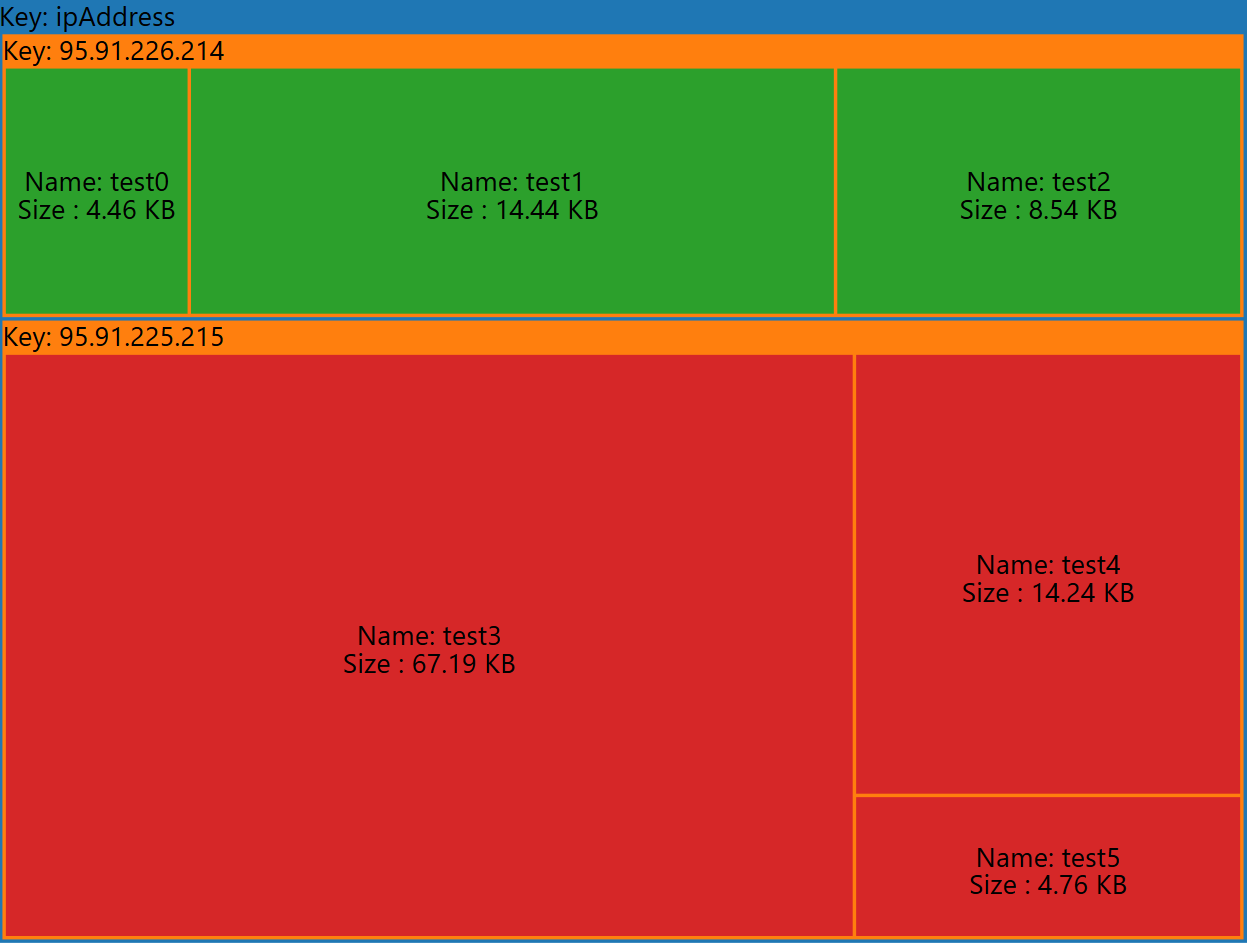
\includegraphics[width=\textwidth]{../pic/IP-Proxy-SetA-tree2.png}
\captionof{figure}{Darstellung der Daten von Alice und Bob}
\end{center}

In Abbildung 3.1 werden die Daten von Alice und Bob dargestellt, welche ohne die Verwendung eines Proxys hochgeladen worden sind. 
\todo{Move this to the end of the text block}

In Abbildung 3.1 sind die IP-Adressen von Alice(95.91.226.214) und Bob(95.91.225.215) erkennbar. 
Zu jeder IP-Adresse können jeweils die drei Dateien der Benutzer zugeordnet werden. 
Die Dateien test0 bis test2 sind der IP-Adresse 95.91.226.214 zugeordnet und test3 bis test5 sind der IP-Adresse 95.91.225.215 zugeordnet.
Damit ist das gegebene Beispiel richtig abgebildet und die echten Relationen zwischen Dateien und IP-Adressen sind richtig modelliert und nachvollziehbar. 

\begin{center}
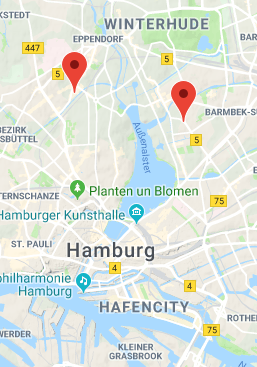
\includegraphics[width=0.5\textwidth]{../pic/IP-Proxy-SetA.png}
\captionof{figure}{Visualisierung von Dateien mittels einer Karte, welche die Geoposition einer IP-Adresse anzeigt}
\end{center}

Die Abbildung 3.2 zeigt uns die Geoposition der IP-Adressen von Alice und Bob und zeigt deren Position in Hamburg, 
wobei die Position nur einen ungefähren Standpunkt darstellt und die eigentliche Position bis zu einem Kilometer abweichen kann.

\begin{center}
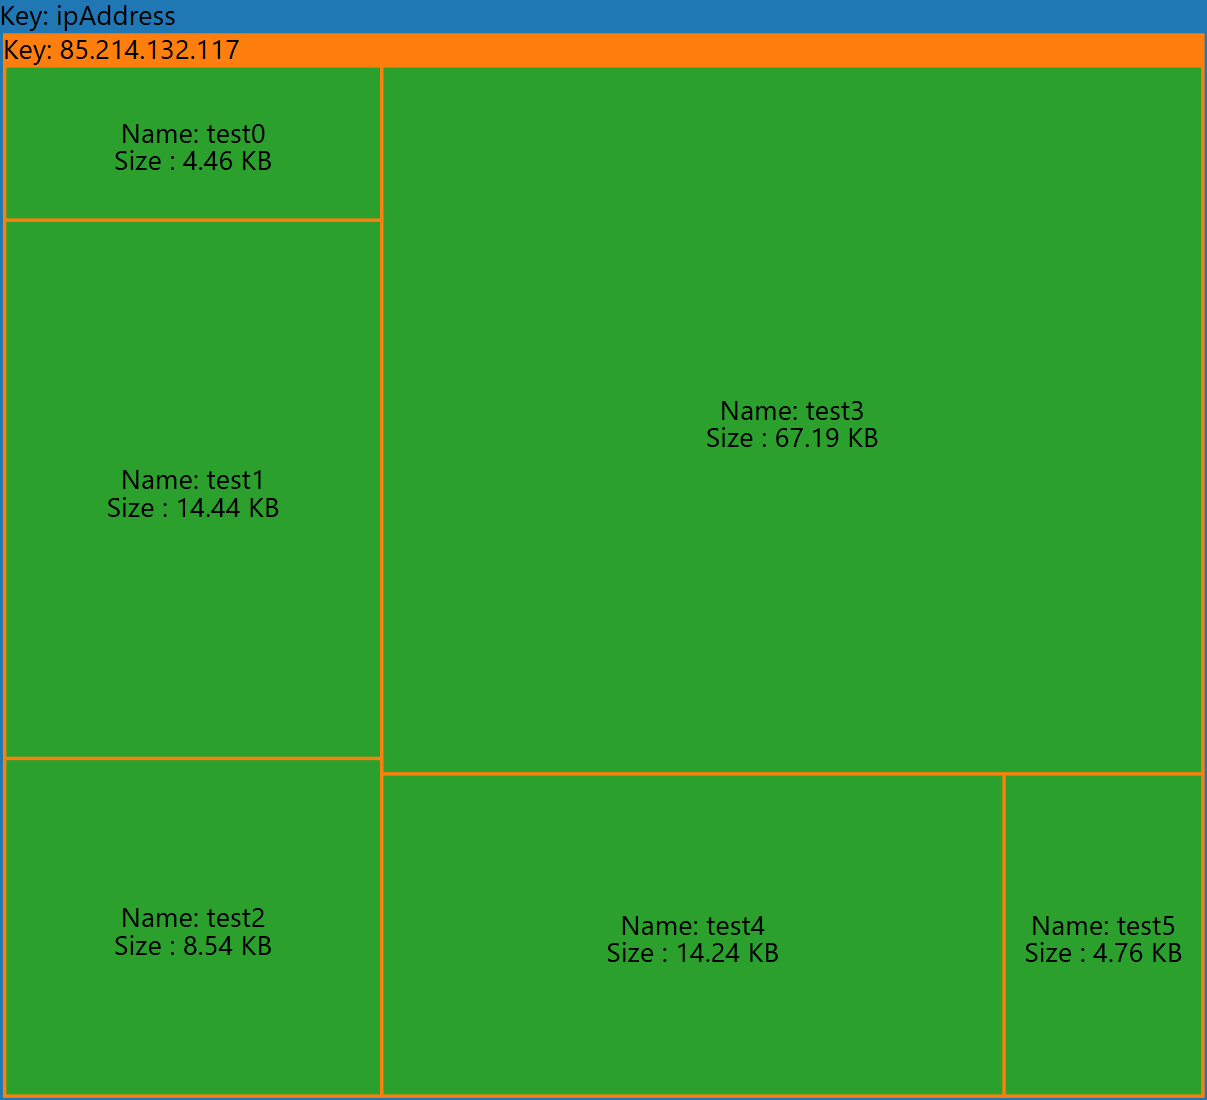
\includegraphics[width=\textwidth]{../pic/IP-Proxy-SetB-tree2.png}\\
\captionof{figure}{Visualisierung von Dateien mittels einer TreeMap, welche nach der IP-Adresse gruppiert sind}
\end{center}

In Abbildung 3.3 sind die Daten visualisiert, welche mittels eines proxy hochgeladen wurden. 
Alle Dateien wurden über die IP-Adresse des proxys 85.214.132.117 gruppiert und somit eine Anonymitätsmenge erzeugt.
Die Daten von Alice und Bob sind nun in einer Anonymitätsmenge zusammengefasst und lassen sich anhand der IP-Adresse nicht mehr eindeutig den beiden Benutzern zuordnen.

\begin{center}
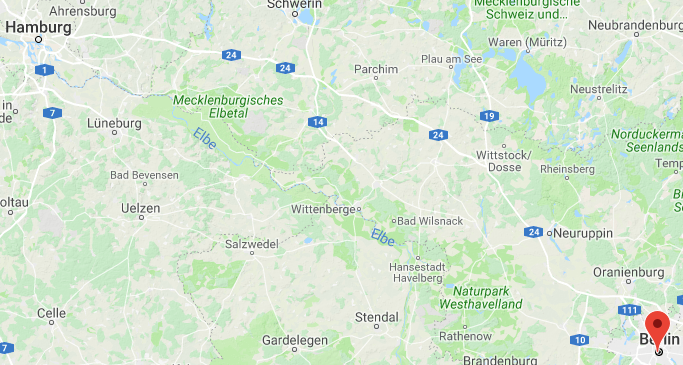
\includegraphics[width=\textwidth]{../pic/IP-Proxy-SetB.png}\\
\captionof{figure}{Visualisierung von Dateien mittels einer Karte, welche die Geoposition einer IP-Adresse anzeigt}
\end{center}

Abbildung 3.4 zeigt und nun die Geoposition des proxys welches in Berlin steht.
Damit sind auch die eigentlichen Geoposition von Alice und Bob durch die Verwendung des Proxys maskiert worden. 

Anstelle eines proxys könnten Alice und Bob das Tor-Netzwerk benutzen um ihre IP-Adressen zu maskieren. Alice und Bob laden drei Dateien, einmal ungeschützt und einmal geschützt durch das Tor-Netzwerk hoch.
Dabei nehmen wir an das alle Dateien einzeln hochgeladen wurden und jeder hochgeladenen Datei eine andere Route durch das Tor-Netzwerk zugewiesen wurde, sodass jede hochgeladene Dateie einen anderen Exit-Server des Tor-Netzwerkes durchläuft. 

\begin{center}
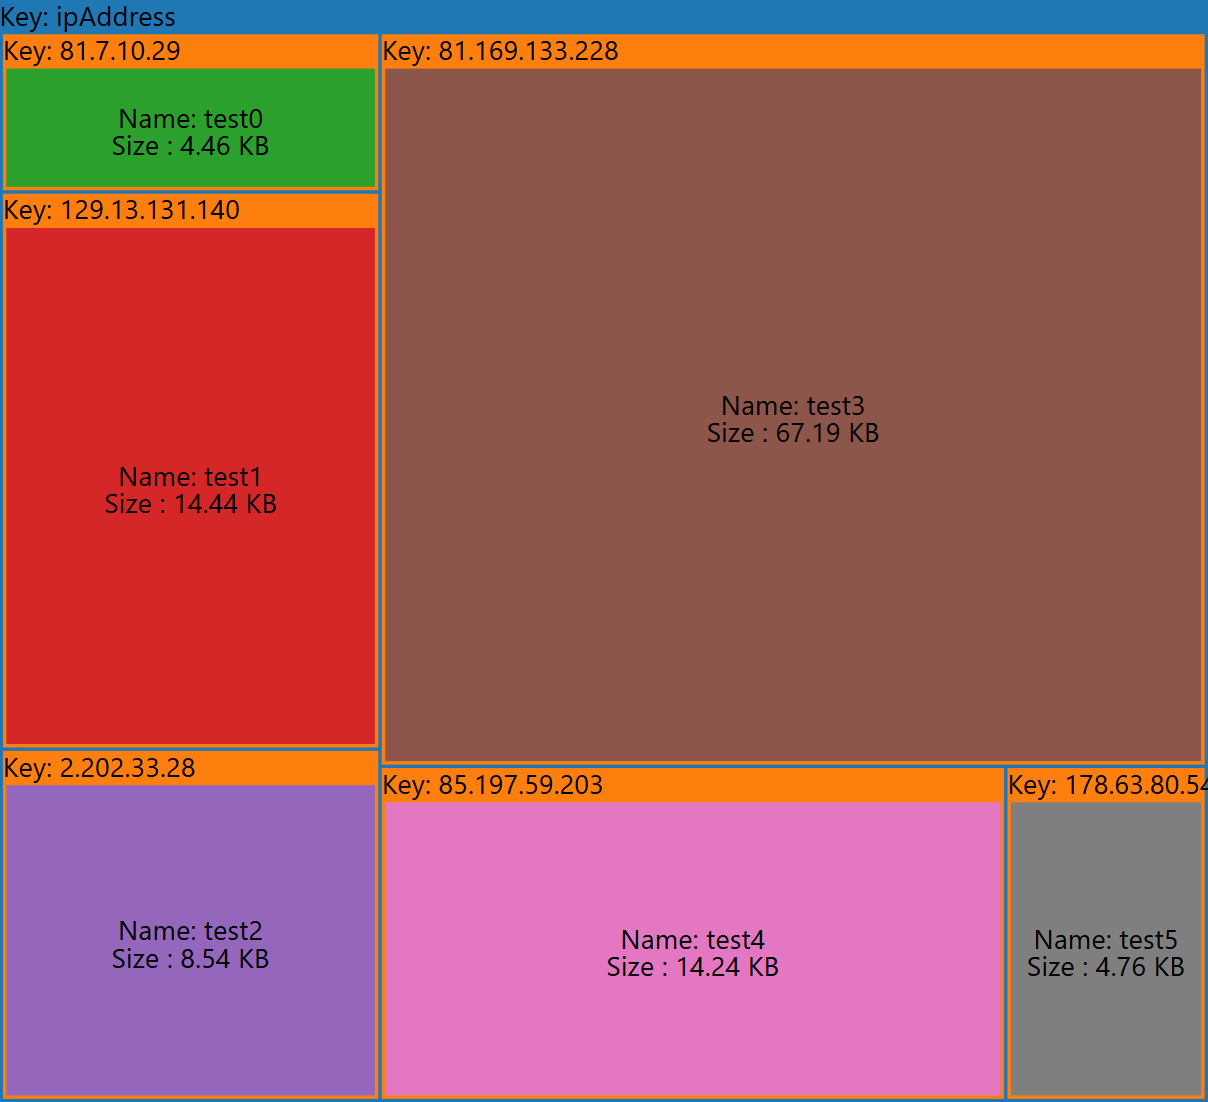
\includegraphics[width=\textwidth]{../pic/IP-Tor-SetB-tree2.png}\\
\captionof{figure}{Visualisierung von Dateien mittels einer TreeMap, welche nach der IP-Adresse gruppiert sind}
\end{center}

In Abbildung 3.5 sehen wir nun die IP-Adressen der verschiedenen Exit-Server des Tor-Netzwerks.
Da jeder hochgeladener Datei ein neuer Exit-Server zugewiesen wurde, können wir über die IP-Adresse die Dateien nicht mehr entsprechend der Benutzer gruppieren.

\begin{center}
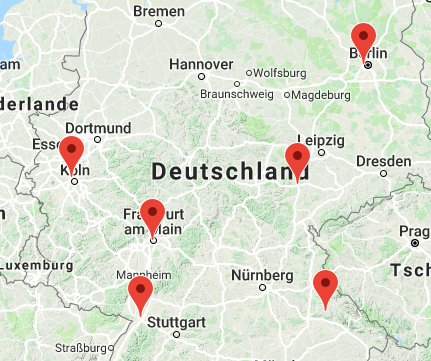
\includegraphics[width=0.7\textwidth]{../pic/IP-Tor-SetB.png}\\
\captionof{figure}{Visualisierung von Dateien mittels einer Karte, welche die Geoposition einer IP-Adresse anzeigt}
\end{center}

Bei Betrachtung der Abbildung 3.6 ist auch erkennbar, das die verschiedenen Positionen der Exit-Server des Tor-Netzwerks variieren und es keinen Anhaltspunkt auf die eigentliche Postion von Alice und Bob gibt. 


\newpage
\section{Darstellung: Headerfingerprinting}

Der Headerfingerprint welcher beim Hochladen der Datei erzeugt wird, wird nun verwendet um die Dateien jeweils  

\newpage
\section{Darstelung: Time Line}
\chapter{Schluss}
\section{Zusammenfassung der Ergebnisse}
\section{kritische Bewertung des Ergebnisse}
\section{neue Problemstellungen, Möglichkeiten zur Weiterführung der Arbeit}
\end{document}
